\section[Geschichte]{Geschichtlicher Verlauf} % (fold)
\label{sec:geschichtlicher_verlauf}
\subsection*{subsection name} % (fold)
\label{sub:subsection_name}

% subsection subsection_name (end)
\begin{frame}
	\frametitle{Geschichtlicher Verlauf}
	\begin{block}{Elektronenmikroskopie}
		\begin{itemize}
			\item 17. Jahrhundert erstes Mikroskop (verstellbare Linse, 40x-240x) 
			\item Mitte 19. Jahrhundert erste Industrielle Herstellung
			\item 1927 Ernst Ruska legt erste Grundsteine.
			\item 1931 Nachweis, dass Objekte in zwei Stufen vergrößert abgebildet werden können.
			\item 1933 Erstes, funktionsfähiges EM (Übermikroskop)
		\end{itemize}
	\end{block}
	\begin{figure}
		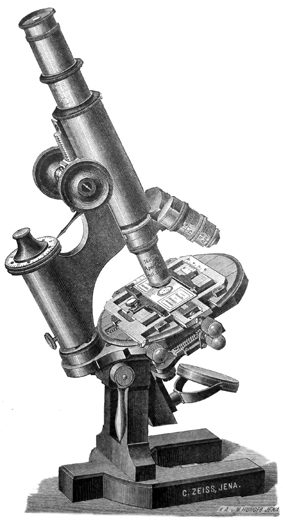
\includegraphics[height = 3cm]{pic/mikroskop1.jpg}
	\end{figure}
\end{frame}

\begin{frame}
	\frametitle{Geschichtlicher Verlauf}
	\begin{block}{Elektronenmikroskopie}
		\begin{itemize}
			\item 1939 erstes Seriengerät mit hoher Bedienungsfreundlichkeit
			\item 1960 Erstmals atomare Auflösung 
			\item 1986 Nobelpreis Physik Ernst Ruska
			\item 1990 Einsatz von Computern
			\item 2005 Vollautomatische Bildaufnahme
		\end{itemize}
	\end{block}
	\begin{figure}
		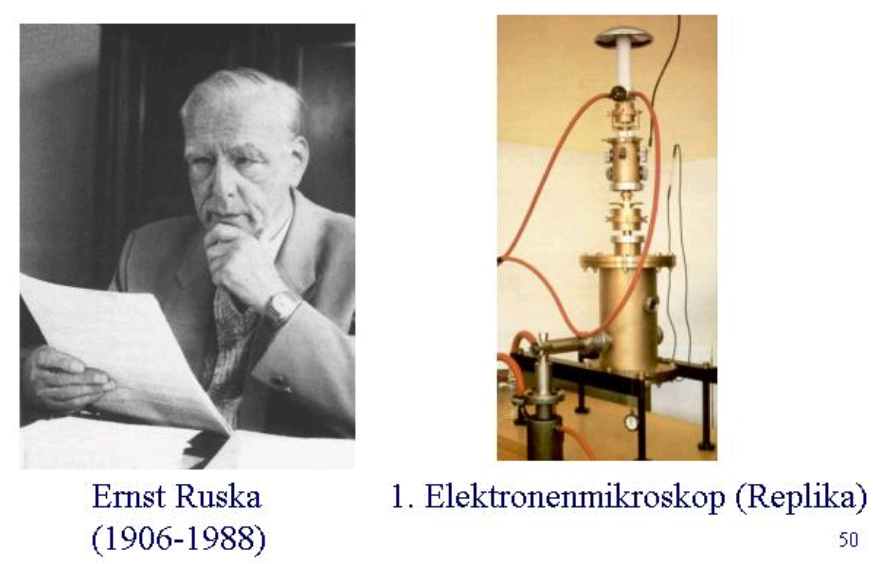
\includegraphics[height = 5cm]{pic/ruska.png}
	\end{figure}
\end{frame}

\begin{frame}
	\frametitle{Geschichtlicher Verlauf}
	\begin{block}{Cryo-TEM}
		\begin{itemize}
			\item 1940 Eis ist nicht Vitrifizierbar
			\item 1960 Erste Forschung an Vitrifiziertem Eis
			\item 1974 Erste mit Stickstoff eingefrorene Probe
			\item 1980 Vitrifizierung mit Ethan
			\item 1986 3.5nm 3D Modell eines Virus
		\end{itemize}
	\end{block}
	"`you cannot bend nature"'
\end{frame}

\begin{frame}
	\frametitle{Geschichtlicher Verlauf}
	\begin{figure}
		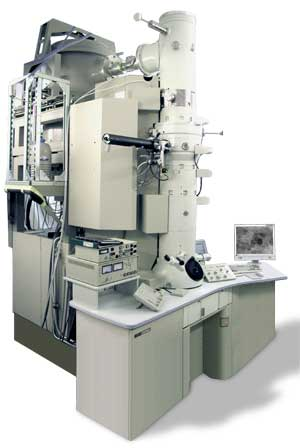
\includegraphics[height = 7cm]{pic/jeol.jpg}
	\end{figure}
\end{frame}